\section{Emil}
\subsection{Overview}
\begin{frame}{Emil: Overview}
\begin{itemize}
  \item Initial Problem and Ideal Scenario
  \item Intelligent Agents
  \item Hardware Choice
\end{itemize}
\end{frame}
 
\subsection{Initial Problem and Ideal Scenario}
\begin{frame}{Intial problem}
\begin{itemize}
\item How can an autonomous turret be designed and constructed such
that it is capable of hitting a moving target.
\end{itemize}
\end{frame}

\begin{frame}{Ideal scenario}
\begin{itemize}
  \item Scanning
  \item Tracking
  \item Shooting
\end{itemize}
\begin{figure}
  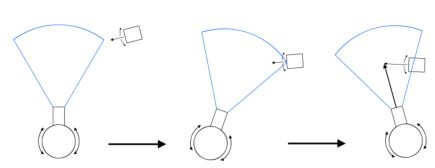
\includegraphics[scale=0.6]{figures/ideal.JPG}
\end{figure}
\end{frame}

\begin{frame}{Embedded Systems}
\begin{itemize}
  \item Single functioned
  \item constrained
  \item reactive
\end{itemize}
\end{frame}

\subsection{Intelligent Agents}
\begin{frame}{Knowledge Representation}
\begin{itemize}
  \item Modelling the problem
  \item Choosing the right kind of solution
\end{itemize}
\begin{figure}
  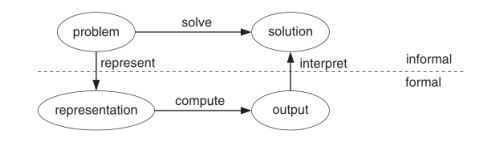
\includegraphics[scale=0.5]{figures/MIRep.JPG}
\end{figure}
\end{frame}

\begin{frame}{Design space}
\begin{itemize}
\item Representation Scheme
\item Planning Horizon
\item Uncertainty
\end{itemize}
\end{frame}

\begin{frame}{Belief Network}
\begin{itemize}
 \item Why choose a Belief Network
 \item Hidden Markov Model
 \begin{figure}
  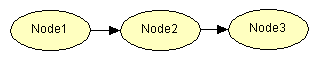
\includegraphics[scale=0.4]{figures/Serial2.PNG}
  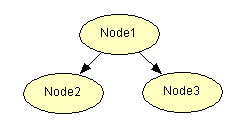
\includegraphics[scale=0.4]{figures/Divergent2.PNG}
  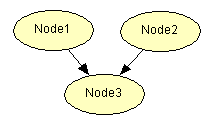
\includegraphics[scale=0.4]{figures/Convergent2.PNG}
\end{figure}
\end{itemize}
\end{frame}

\subsection{Hardware choice}
\begin{frame}{Platform Choice}
\begin{itemize}
 \item LEGO Mindstorms NXT
 \item Arduino
\end{itemize}
\end{frame}

\begin{frame}{Sensor Choice}
\begin{itemize}
 \item Ultrasonic sensor
 \item Camera
\end{itemize}
\end{frame}
 
